\documentclass[a4paper, 11pt]{article}
\usepackage{graphicx}
\usepackage{multicol}
\usepackage{tabularx}
\usepackage{enumitem}
\usepackage[a4paper, margin=1.8cm]{geometry}
\usepackage{listings}
\usepackage{amssymb}
\usepackage{gvv}
\usepackage{gvv-book}
\usepackage{amsmath}
\usepackage{setspace}
\usepackage{caption}

\graphicspath{./figs/}

\begin{document}
\begin{center}
    \huge{EC : ELECTRONICS AND COMMUNICATION ENGINEERING}\\
    \large{EE25BTECH11041 - Naman Kumar}
\end{center}
\begin{enumerate}
\section*{General Aptitude (GA)}
    \item "By giving him the last \underline{\hspace{2cm}} of the cake, you will ensure lasting \underline{\hspace{2cm}} in our house today."
    The words that best fill the blanks in the above sentence are
    \begin{enumerate}
        \begin{multicols}{2}
            \item peas, piece
            \item piece, peace
            \item peace, piece
            \item peace, peas
        \end{multicols}
    \end{enumerate}

    \hfill{\brak{\text{GATE EC 2018}}}

    \item "Even though there is a vast scope for its \underline{\hspace{2cm}}, tourism has remained a/an \underline{\hspace{2cm}} area."
    The words that best fill the blanks in the above sentence are
    \begin{enumerate}
        \begin{multicols}{2}
            \item improvement, neglected
            \item rejection, approved
            \item fame, glum
            \item interest, disinterested
        \end{multicols}
    \end{enumerate}

    \hfill{\brak{\text{GATE EC 2018}}}

    \item If the number 715\underline{\hspace{0.5cm}}423 is divisible by 3 \brak{\underline{\hspace{0.5cm}} denotes the missing digit in the thousandths place}, then the smallest whole number in the place of \underline{\hspace{0.5cm}} is
    \begin{enumerate}
        \begin{multicols}{4}
            \item 0
            \item 2
            \item 5
            \item 6
        \end{multicols}
    \end{enumerate}

    \hfill{\brak{\text{GATE EC 2018}}}

    \item What is the value of $1+\frac{1}{4}+\frac{1}{16}+\frac{1}{64}+\frac{1}{256}+\dots$?
    \begin{enumerate}
        \begin{multicols}{4}
            \item 2
            \item $\frac{7}{4}$
            \item $\frac{3}{2}$
            \item $\frac{4}{3}$
        \end{multicols}
    \end{enumerate}

    \hfill{\brak{\text{GATE EC 2018}}}

    \item A 1.5 m tall person is standing at a distance of 3 m from a lamp post. The light from the lamp at the top of the post casts her shadow. The length of the shadow is twice her height. What is the height of the lamp post in meters?
    \begin{enumerate}
        \begin{multicols}{4}
            \item 1.5
            \item 3
            \item 4.5
            \item 6
        \end{multicols}
    \end{enumerate}

    \hfill{\brak{\text{GATE EC 2018}}}

    \item Leila aspires to buy a car worth Rs. 10,00,000 after 5 years. What is the minimum amount in Rupees that she should deposit now in a bank which offers 10\% annual rate of interest, if the interest was compounded annually?
    \begin{enumerate}
        \begin{multicols}{2}
            \item 5,00,000
            \item 6,21,000
            \item 6,66,667
            \item 7,50,000
        \end{multicols}
    \end{enumerate}

    \hfill{\brak{\text{GATE EC 2018}}}

    \item Two alloys A and B contain gold and copper in the ratios of 2:3 and 3:7 by mass, respectively. Equal masses of alloys A and B are melted to make an alloy C. The ratio of gold to copper in alloy C is
    \begin{enumerate}
        \begin{multicols}{4}
            \item 5:10
            \item 7:13
            \item 6:11
            \item 9:13
        \end{multicols}
    \end{enumerate}

    \hfill{\brak{\text{GATE EC 2018}}}

    \item The Cricket Board has long recognized John's potential as a leader of the team. However, his on-field temper has always been a matter of concern for them since his junior days. While this aggression has filled stadia with die-hard fans, it has taken a toll on his own batting. Until recently, it appeared that he found it difficult to convert his aggression into big scores. Over the past three seasons though, that picture of John has been replaced by a cerebral, calculative and successful batsman-captain. After many years, it appears that the team has finally found a complete captain.
    Which of the following statements can be logically inferred from the above paragraph?
    \begin{enumerate}[label=(\roman*)]
        \item Even as a junior cricketer, John was considered a good captain.
        \item Finding a complete captain is a challenge.
        \item Fans and the Cricket Board have differing views on what they want in a captain.
        \item Over the past three seasons John has accumulated big scores.
    \end{enumerate}
    \begin{enumerate}
        \item (i), (ii) and (iii) only
        \item (iii) and (iv) only
        \item (ii) and (iv) only
        \item (i), (ii), (iii) and (iv)
    \end{enumerate}

    \hfill{\brak{\text{GATE EC 2018}}}

    \item A cab was involved in a hit and run accident at night. You are given the following data about the cabs in the city and the accident.
    \begin{enumerate}[label=(\roman*)]
        \item 85\% of cabs in the city are green and the remaining cabs are blue.
        \item A witness identified the cab involved in the accident as blue.
        \item It is known that a witness can correctly identify the cab colour only 80\% of the time.
    \end{enumerate}
    Which of the following options is closest to the probability that the accident was caused by a blue cab?
    \begin{enumerate}
        \begin{multicols}{4}
            \item 12\%
            \item 15\%
            \item 41\%
            \item 80\%
        \end{multicols}
    \end{enumerate}

    \hfill{\brak{\text{GATE EC 2018}}}

    \item A coastal region with unparalleled beauty is home to many species of animals. It is dotted with coral reefs and unspoilt white sandy beaches. It has remained inaccessible to tourists due to poor connectivity and lack of accommodation. A company has spotted the opportunity and is planning to develop a luxury resort with helicopter service to the nearest major city airport. Environmentalists are upset that this would lead to the region becoming crowded and polluted like any other major beach resorts.
    Which one of the following statements can be logically inferred from the information given in the above paragraph?
    \begin{enumerate}
        \item The culture and tradition of the local people will be influenced by the tourists.
        \item The region will become crowded and polluted due to tourism.
        \item The coral reefs are on the decline and could soon vanish.
        \item Helicopter connectivity would lead to an increase in tourists coming to the region.
    \end{enumerate}

    \hfill{\brak{\text{GATE EC 2018}}}
\end{enumerate}


\begin{enumerate}
\section*{Electronics and Communication Engineering \brak{EC}}
    \item Two identical nMOS transistors $M_1$ and $M_2$ are connected as shown below. The circuit is used as an amplifier with the input connected between G and S terminals and the output taken between D and S terminals. $V_{bias}$ and $V_D$ are so adjusted that both transistors are in saturation. The transconductance of this combination is defined as $g_m = \frac{\partial i_D}{\partial v_{GS}}$ where $i_D$ is the current flowing into the drain of $M_2$. Let $g_{m1}, g_{m2}$ be the transconductances and $r_{o1}, r_{o2}$ be the output resistances of transistors $M_1$ and $M_2$, respectively.
    
    \begin{figure}[H]
        \centering
        \includegraphics[width=0.4\columnwidth]{figs/q1.png}
        \caption*{}
        \label{fig:q1}
    \end{figure}
    Which of the following statements about estimates for $g_m$ and $r_o$ is correct?
    \begin{enumerate}
        \item $g_m \approx g_{m1} \cdot g_{m2} \cdot r_{o2}$ and $r_o \approx r_{o1} + r_{o2}$.
        \item $g_m \approx g_{m1} + g_{m2}$ and $r_o \approx r_{o1} + r_{o2}$.
        \item $g_m \approx g_{m1}$ and $r_o \approx r_{o1} \cdot g_{m2} \cdot r_{o2}$.
        \item $g_m \approx g_{m1}$ and $r_o \approx r_{o2}$.
    \end{enumerate}

    \hfill{\brak{\text{GATE EC 2018}}}

    \item In the circuit shown below, the op-amp is ideal and Zener voltage of the diode is $2.5$ volts. At the input, unit step voltage is applied, i.e. $v_{IN}\brak{t} = u\brak{t}$ volts. Also, at $t=0$, the voltage across each of the capacitors is zero.

    \begin{figure}[H]
        \centering
        \includegraphics[width=0.6\columnwidth]{figs/q2.png}
        \caption*{}
        \label{fig:q2}
    \end{figure}
    The time t, in milliseconds, at which the output voltage $v_{OUT}$ crosses -10 V is
    \begin{enumerate}
        \begin{multicols}{4}
            \item $2.5$
            \item $5$
            \item $7.5$
            \item $10$
        \end{multicols}
    \end{enumerate}

    \hfill{\brak{\text{GATE EC 2018}}}

    \item A good transimpedance amplifier has
    \begin{enumerate}
        \item low input impedance and high output impedance.
        \item high input impedance and high output impedance.
        \item high input impedance and low output impedance.
        \item low input impedance and low output impedance.
    \end{enumerate}

    \hfill{\brak{\text{GATE EC 2018}}}

    \item Let the input be u and the output be y of a system, and the other parameters are real constants. Identify which among the following systems is not a linear system:
    \begin{enumerate}
        \item $\frac{d^2y}{dt^2} + a_1\frac{dy}{dt} + a_2y = b_2\frac{d^2u}{dt^2} + b_1\frac{du}{dt} + b_0u$ \brak{\text{with initial rest conditions}}
        \item $y\brak{t} = \int_{0}^{t} e^{\alpha\brak{t-\tau}} \beta u\brak{\tau} d\tau$
        \item $y = au + b$, $b \ne 0$
        \item $y = au$
    \end{enumerate}

    \hfill{\brak{\text{GATE EC 2018}}}

    \item The Nyquist stability criterion and the Routh criterion both are powerful analysis tools for determining the stability of feedback controllers. Identify which of the following statements is FALSE:
    \begin{enumerate}
        \item Both the criteria provide information relative to the stable gain range of the system.
        \item The general shape of the Nyquist plot is readily obtained from the Bode magnitude plot for all minimum-phase systems.
        \item The Routh criterion is not applicable in the condition of transport lag, which can be readily handled by the Nyquist criterion.
        \item The closed-loop frequency response for a unity feedback system cannot be obtained from the Nyquist plot.
    \end{enumerate}

    \hfill{\brak{\text{GATE EC 2018}}}

    \item Consider $p\brak{s} = s^3 + a_2s^2 + a_1s + a_0$ with all real coefficients. It is known that its derivative $p'\brak{s}$ has no real roots. The number of real roots of $p\brak{s}$ is
    \begin{enumerate}
        \begin{multicols}{4}
            \item $0$
            \item $1$
            \item $2$
            \item $3$
        \end{multicols}
    \end{enumerate}

    \hfill{\brak{\text{GATE EC 2018}}}

    \item In a p-n junction diode at equilibrium, which one of the following statements is NOT TRUE?
    \begin{enumerate}
        \item The hole and electron diffusion current components are in the same direction.
        \item The hole and electron drift current components are in the same direction.
        \item On an average, holes and electrons drift in opposite direction.
        \item On an average, electrons drift and diffuse in the same direction.
    \end{enumerate}

    \hfill{\brak{\text{GATE EC 2018}}}
    
    \item The logic function $f\brak{X,Y}$ realized by the given circuit is
    \begin{figure}[H]
        \centering
        \includegraphics[width=0.5\columnwidth]{figs/q8.png}
        \caption*{}
        \label{fig:q8}
    \end{figure}
    \begin{enumerate}
        \begin{multicols}{4}
            \item NOR
            \item AND
            \item NAND
            \item XOR
        \end{multicols}
    \end{enumerate}

    \hfill{\brak{\text{GATE EC 2018}}}

    \item A function $F\brak{A,B,C}$ defined by three Boolean variables A, B and C when expressed as sum of products is given by\\$F = \overline{A} \cdot \overline{B} \cdot \overline{C} + \overline{A} \cdot B \cdot \overline{C} + A \cdot \overline{B} \cdot \overline{C}$\\where, $\overline{A}, \overline{B}$, and $\overline{C}$ are the complements of the respective variables. The product of sums \brak{POS} form of the function F is
    \begin{enumerate}
        \item $F = \brak{A+B+C} \cdot \brak{A+\overline{B}+C} \cdot \brak{\overline{A}+B+C}$
        \item $F = \brak{\overline{A}+\overline{B}+\overline{C}} \cdot \brak{\overline{A}+B+\overline{C}} \cdot \brak{A+\overline{B}+\overline{C}}$
        \item $F = \brak{A+B+\overline{C}} \cdot \brak{A+\overline{B}+\overline{C}} \cdot \brak{\overline{A}+B+\overline{C}} \cdot \brak{\overline{A}+\overline{B}+C} \cdot \brak{\overline{A}+\overline{B}+\overline{C}}$
        \item $F = \brak{\overline{A}+\overline{B}+C} \cdot \brak{\overline{A}+B+C} \cdot \brak{A+\overline{B}+C} \cdot \brak{A+B+\overline{C}} \cdot \brak{A+B+C}$
    \end{enumerate}

    \hfill{\brak{\text{GATE EC 2018}}}

    \item The points P, Q, and R shown on the Smith chart \brak{normalized impedance chart} in the following figure represent:
    \begin{figure}[H]
        \centering
        \includegraphics[width=0.4\columnwidth]{figs/q10.png}
        \caption*{}
        \label{fig:q10}
    \end{figure}
    \begin{enumerate}
        \item P: Open Circuit, Q: Short Circuit, R: Matched Load
        \item P: Open Circuit, Q: Matched Load, R: Short Circuit
        \item P: Short Circuit, Q: Matched Load, R: Open Circuit
        \item P: Short Circuit, Q: Open Circuit, R: Matched Load
    \end{enumerate}

    \hfill{\brak{\text{GATE EC 2018}}}

    \item Let M be a real $4 \times 4$ matrix. Consider the following statements:\\
    \begin{tabular}{ll}
        S1: & M has 4 linearly independent eigenvectors. \\
        S2: & M has 4 distinct eigenvalues.\\
        S3: & M is non-singular \brak{invertible}.
    \end{tabular}\\
    Which one among the following is TRUE?
    \begin{enumerate}
        \begin{multicols}{2}
            \item S1 implies S2
            \item S1 implies S3
            \item S2 implies S1
            \item S3 implies S2
        \end{multicols}
    \end{enumerate}

    \hfill{\brak{\text{GATE EC 2018}}}

    \item Let $f\brak{x,y} = \frac{ax^2+by^2}{xy}$, where a and b are constants. If at $x=1$ and $y=2$, $\frac{\partial f}{\partial x} = \frac{\partial f}{\partial y}$, then the relation between a and b is
    \begin{enumerate}
        \begin{multicols}{4}
            \item $a = \frac{b}{4}$
            \item $a = \frac{b}{2}$
            \item $a = 2b$
            \item $a = 4b$
        \end{multicols}
    \end{enumerate}

    \hfill{\brak{\text{GATE EC 2018}}}

    \item A discrete-time all-pass system has two of its poles at $0.25\angle0^{\circ}$ and $2\angle30^{\circ}$. Which one of the following statements about the system is TRUE?
    \begin{enumerate}
        \item It has two more poles at $0.5\angle30^{\circ}$ and $4\angle0^{\circ}$.
        \item It is stable only when the impulse response is two-sided.
        \item It has constant phase response over all frequencies.
        \item It has constant group delay over all frequencies.
    \end{enumerate}

    \hfill{\brak{\text{GATE EC 2018}}}
    
    \item Let $x\brak{t}$ be a periodic function with period $T=10$. The Fourier series coefficients for this series are denoted by $a_k$, that is
    \begin{center}
        $x\brak{t} = \sum_{k=-\infty}^{\infty} a_k e^{ik\frac{2\pi}{T}t}$. 
    \end{center}
    The same function $x\brak{t}$ can also be considered as a periodic function with period $T' = 40$. Let $b_k$ be the Fourier series coefficients when period is taken as $T'$. If $\sum_{k=-\infty}^{\infty} |a_k| = 16$, then $\sum_{k=-\infty}^{\infty} |b_k|$ is equal to
    \begin{enumerate}
        \begin{multicols}{4}
            \item $256$
            \item $64$
            \item $16$
            \item $4$
        \end{multicols}
    \end{enumerate}

    \hfill{\brak{\text{GATE EC 2018}}}

    \item Consider the following amplitude modulated signal: 
    \begin{center}
    $s\brak{t} = \cos\brak{2000\pi t} + 4\cos\brak{2400\pi t} + \cos\brak{2800\pi t}$. 
    \end{center}
    The ratio \brak{\text{accurate to three decimal places}} of the power of the message signal to the power of the carrier signal is \underline{\hspace{2cm}}.

    \hfill{\brak{\text{GATE EC 2018}}}
    
    \item Consider a binary channel code in which each codeword has a fixed length of 5 bits. The Hamming distance between any pair of distinct codewords in this code is at least 2. The maximum number of codewords such a code can contain is \underline{\hspace{2cm}}.

    \hfill{\brak{\text{GATE EC 2018}}}

    \item A binary source generates symbols $X \in \{-1, 1\}$ which are transmitted over a noisy channel. The probability of transmitting $X=1$ is $0.5$. Input to the threshold detector is $R = X + N$. The probability density function $f_N\brak{n}$ of the noise N is shown below.
    \begin{figure}[H]
        \centering
        \includegraphics[width=0.5\columnwidth]{figs/q17.png}
        \caption*{}
        \label{fig:q17}
    \end{figure}
    If the detection threshold is zero, then the probability of error \brak{\text{correct to two decimal places}} is \underline{\hspace{2cm}}.

    \hfill{\brak{\text{GATE EC 2018}}}
    
    \item A p-n step junction diode with a contact potential of $0.65$ V has a depletion width of $1$ $\mu$m at equilibrium. The forward voltage \brak{\text{in volts, correct to two decimal places}} at which this width reduces to $0.6$ $\mu$m is \underline{\hspace{2cm}}.

    \hfill{\brak{\text{GATE EC 2018}}}
    
    \item A traffic signal cycles from GREEN to YELLOW, YELLOW to RED and RED to GREEN. In each cycle, GREEN is turned on for 70 seconds, YELLOW is turned on for 5 seconds and the RED is turned on for 75 seconds. This traffic light has to be implemented using a finite state machine \brak{FSM}. The only input to this FSM is a clock of 5 second period. The minimum number of flip-flops required to implement this FSM is \underline{\hspace{2cm}}.

    \hfill{\brak{\text{GATE EC 2018}}}

    \item There are two photolithography systems: one with light source of wavelength $\lambda_1 = 156$ nm \brak{System 1} and another with light source of wavelength $\lambda_2 = 325$ nm \brak{System 2}. Both photolithography systems are otherwise identical. If the minimum feature sizes that can be realized using System 1 and System 2 are $L_{min1}$ and $L_{min2}$ respectively, the ratio $L_{min1}/L_{min2}$ \brak{\text{correct to two decimal places}} is \underline{\hspace{2cm}}.
    
    \hfill{\brak{\text{GATE EC 2018}}}

    \item A lossy transmission line has resistance per unit length $R = 0.05$ $\Omega$/m. The line is distortionless and has characteristic impedance of 50 $\Omega$. The attenuation constant \brak{\text{in Np/m, correct to three decimal places}} of the line is \underline{\hspace{2cm}}.

    \hfill{\brak{\text{GATE EC 2018}}}

    \item Consider matrix $A = \myvec{k & 2k \\ k^2-k & k^2}$ and vector $x = \myvec{x_1 \\ x_2}$. The number of distinct real values of k for which the equation $Ax=0$ has infinitely many solutions is \underline{\hspace{2cm}}.

    \hfill{\brak{\text{GATE EC 2018}}}
    
    \item Let $X_1, X_2, X_3$ and $X_4$ be independent normal random variables with zero mean and unit variance. The probability that $X_4$ is the smallest among the four is \underline{\hspace{2cm}}.

    \hfill{\brak{\text{GATE EC 2018}}}

    \item Taylor series expansion of $f\brak{x} = \int_{0}^{x} e^{-\brak{\frac{t^2}{2}}} dt$ around $x=0$ has the form $f\brak{x} = a_0 + a_1x + a_2x^2 + \dots$. The coefficient $a_2$ \brak{\text{correct to two decimal places}} is equal to \underline{\hspace{2cm}}.
    
    \hfill{\brak{\text{GATE EC 2018}}}

    \item The ABCD matrix for a two-port network is defined by:
    \[ \myvec{V_1 \\ I_1} = \myvec{A & B \\ C & D} \myvec{V_2 \\ -I_2} \]
    \begin{figure}[H]
        \centering
        \includegraphics[width=0.6\columnwidth]{figs/q25.png}
        \caption*{}
        \label{fig:q25}
    \end{figure}
    The parameter B for the given two-port network \brak{\text{in ohms, correct to two decimal places}} is \underline{\hspace{2cm}}.

    \hfill{\brak{\text{GATE EC 2018}}}

    \item The circuit shown in the figure is used to provide regulated voltage \brak{5 V} across the 1k$\Omega$ resistor. Assume that the Zener diode has a constant reverse breakdown voltage for a current range, starting from a minimum required Zener current, $I_{zmin} = 2$ mA to its maximum allowable current. The input voltage $V_I$ may vary by 5\% from its nominal value of 6 V. The resistance of the diode in the breakdown region is negligible.
    \begin{figure}[H]
        \centering
        \includegraphics[width=0.5\columnwidth]{figs/q26.png}
        \caption*{}
        \label{fig:q26}
    \end{figure}
    The value of R and the minimum required power dissipation rating of the diode, respectively, are
    \begin{enumerate}
        \begin{multicols}{2}
            \item 186 $\Omega$ and 10 mW
            \item 100 $\Omega$ and 40 mW
            \item 100 $\Omega$ and 10 mW
            \item 186 $\Omega$ and 40 mW
        \end{multicols}
    \end{enumerate}

    \hfill{\brak{\text{GATE EC 2018}}}

    \item Let $c\brak{t}=A_c\cos\brak{2\pi f_c t}$ and $m\brak{t}=\cos\brak{2\pi f_m t}$. It is given that $f_c \gg 5f_m$. The signal $c\brak{t}+m\brak{t}$ is applied to the input of a non-linear device, whose output $v_o\brak{t}$ is related to the input $v_i\brak{t}$ as $v_o\brak{t} = av_i\brak{t} + bv_i^2\brak{t}$, where a and b are positive constants. The output of the non-linear device is passed through an ideal band-pass filter with center frequency $f_c$ and bandwidth $3f_m$ to produce an amplitude modulated \brak{AM} wave. If it is desired to have the sideband power of the AM wave to be half of the carrier power, then $a/b$ is
    \begin{enumerate}
        \begin{multicols}{4}
            \item 0.25
            \item 0.5
            \item 1
            \item 2
        \end{multicols}
    \end{enumerate}

    \hfill{\brak{\text{GATE EC 2018}}}

    \item Consider a white Gaussian noise process $N\brak{t}$ with two-sided power spectral density $S_N\brak{f}=0.5$ W/Hz as input to a filter with impulse response $0.5e^{-t^2/2}$ \brak{where t is in seconds} resulting in output $Y\brak{t}$. The power in $Y\brak{t}$ in watts is
    \begin{enumerate}
        \begin{multicols}{4}
            \item 0.11
            \item 0.22
            \item 0.33
            \item 0.44
        \end{multicols}
    \end{enumerate}

    \hfill{\brak{\text{GATE EC 2018}}}

    \item The state equation and the output equation of a control system are given below:
    \[ \dot{x} = \myvec{-4 & -1.5 \\ 4 & 0} x + \myvec{2 \\ 0} u. \]
    \[ y = \myvec{1.5 & 0.625} x \]
    The transfer function representation of the system is
    \begin{enumerate}
        \begin{multicols}{2}
            \item $\frac{3s+5}{s^2+4s+6}$
            \item $\frac{3s-1.875}{s^2+4s+6}$
            \item $\frac{4s+1.5}{s^2+4s+6}$
            \item $\frac{6s+5}{s^2+4s+6}$
        \end{multicols}
    \end{enumerate}

    \hfill{\brak{\text{GATE EC 2018}}}

    \item Red \brak{R}, Green \brak{G} and Blue \brak{B} Light Emitting Diodes \brak{LEDs} were fabricated using p-n junctions of three different inorganic semiconductors having different band-gaps. The built-in voltages of red, green and blue diodes are $V_R$, $V_G$ and $V_B$, respectively. Assume donor and acceptor doping to be the same \brak{$N_A$ and $N_D$ respectively} in the p and n sides of all the three diodes.
    Which one of the following relationships about the built-in voltages is TRUE?
    \begin{enumerate}
        \begin{multicols}{2}
            \item $V_R > V_G > V_B$
            \item $V_R < V_G < V_B$
            \item $V_R = V_G = V_B$
            \item $V_R > V_G < V_B$
        \end{multicols}
    \end{enumerate}

    \hfill{\brak{\text{GATE EC 2018}}}

    \item A four-variable Boolean function is realized using $4 \times 1$ multiplexers as shown in the figure.
    \begin{figure}[H]
        \centering
        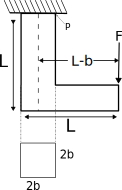
\includegraphics[width=0.8\columnwidth]{figs/q31.png}
        \caption*{}
        \label{fig:q31}
    \end{figure}
    The minimized expression for $F\brak{U,V,W,X}$ is
    \begin{enumerate}
        \begin{multicols}{2}
            \item $\brak{UV + \overline{U}\overline{V}}\overline{W}$
            \item $\brak{UV + \overline{U}\overline{V}}\brak{\overline{W}\overline{X} + \overline{W}X}$
            \item $\brak{U\overline{V} + \overline{U}V}\overline{W}$
            \item $\brak{U\overline{V} + \overline{U}V}\brak{\overline{W}\overline{X} + \overline{W}X}$
        \end{multicols}
    \end{enumerate}
    
    \hfill{\brak{\text{GATE EC 2018}}}

    \item A $2 \times 2$ ROM array is built with the help of diodes as shown in the circuit below. Here W0 and W1 are signals that select the word lines and B0 and B1 are signals that are output of the sense amps based on the stored data corresponding to the bit lines during the read operation.
    \begin{figure}[H]
        \centering
        \includegraphics[width=0.5\columnwidth]{figs/q32.png}
        \caption*{}
        \label{fig:q32}
    \end{figure}
    During the read operation, the selected word line goes high and the other word line is in a high impedance state. As per the implementation shown in the circuit diagram above, what are the bits corresponding to $D_{ij}$ \brak{where $i=0$ or 1 and $j=0$ or 1} stored in the ROM?
    \begin{enumerate}
        \begin{multicols}{2}
            \item $\myvec{1 & 0 \\ 0 & 1}$
            \item $\myvec{0 & 1 \\ 1 & 0}$
            \item $\myvec{1 & 0 \\ 1 & 0}$
            \item $\myvec{1 & 1 \\ 0 & 0}$
        \end{multicols}
    \end{enumerate}

    \hfill{\brak{\text{GATE EC 2018}}}

    \item The distance \brak{in meters} a wave has to propagate in a medium having a skin depth of 0.1 m so that the amplitude of the wave attenuates by 20 dB, is
    \begin{enumerate}
        \begin{multicols}{4}
            \item 0.12
            \item 0.23
            \item 0.46
            \item 2.3
        \end{multicols}
    \end{enumerate}

    \hfill{\brak{\text{GATE EC 2018}}}

    \item A curve passes through the point $\brak{x=1, y=0}$ and satisfies the differential equation $\frac{dy}{dx} = \frac{x^2+y^2}{2y} + \frac{y}{x}$. The equation that describes the curve is
    \begin{enumerate}
        \item $\ln\brak{1+\frac{y^2}{x^2}} = x-1$
        \item $\frac{1}{2}\ln\brak{1+\frac{y^2}{x^2}} = x-1$
        \item $\ln\brak{1+\frac{y}{x}} = x-1$
        \item $\frac{1}{2}\ln\brak{1+\frac{y}{x}} = x-1$
    \end{enumerate}

    \hfill{\brak{\text{GATE EC 2018}}}

    \item For the circuit given in the figure, the voltage $V_c$ \brak{in volts} across the capacitor is
    \begin{figure}[H]
        \centering
        \includegraphics[width=0.6\columnwidth]{figs/q35.png}
        \caption*{}
        \label{fig:q35}
    \end{figure}
    \begin{enumerate}
        \begin{multicols}{2}
            \item $1.25\sqrt{2}\sin\brak{5t - 0.25\pi}$
            \item $1.25\sqrt{2}\sin\brak{5t - 0.125\pi}$
            \item $2.5\sqrt{2}\sin\brak{5t - 0.25\pi}$
            \item $2.5\sqrt{2}\sin\brak{5t - 0.125\pi}$
        \end{multicols}
    \end{enumerate}

    \hfill{\brak{\text{GATE EC 2018}}}

    \item For the circuit given in the figure, the magnitude of the loop current \brak{in amperes, correct to three decimal places} 0.5 second after closing the switch is \underline{\hspace{2cm}}.
    \begin{figure}[H]
        \centering
        \includegraphics[width=0.6\columnwidth]{figs/q36.png}
        \caption*{}
        \label{fig:q36}
    \end{figure}

    \hfill{\brak{\text{GATE EC 2018}}}

    \item A dc current of 26 $\mu$A flows through the circuit shown. The diode in the circuit is forward biased and it has an ideality factor of one. At the quiescent point, the diode has a junction capacitance of 0.5 nF. Its neutral region resistances can be neglected. Assume that the room temperature thermal equivalent voltage is 26 mV.
    \begin{figure}[H]
        \centering
        \includegraphics[width=0.5\columnwidth]{figs/q37.png}
        \caption*{}
        \label{fig:q37}
    \end{figure}
    For $\omega = 2 \times 10^6$ rad/s, the amplitude of the small-signal component of diode current \brak{in $\mu$A, correct to one decimal place} is \underline{\hspace{2cm}}.

    \hfill{\brak{\text{GATE EC 2018}}}

    \item An op-amp based circuit is implemented as shown below.
    \begin{figure}[H]
        \centering
        \includegraphics[width=0.6\columnwidth]{figs/q38.png}
        \caption*{}
        \label{fig:q38}
    \end{figure}
    In the above circuit, assume the op-amp to be ideal. The voltage \brak{\text{in volts, correct to one decimal place}} at node A, connected to the negative input of the op-amp as indicated in the figure is \underline{\hspace{2cm}}.

    \hfill{\brak{\text{GATE EC 2018}}}

    \item The input 4sinc\brak{2t} is fed to a Hilbert transformer to obtain $y\brak{t}$, as shown in the figure below:
    \begin{figure}[H]
        \centering
        \includegraphics[width=0.5\columnwidth]{figs/q39.png}
        \caption*{}
        \label{fig:q39}
    \end{figure}
    Here sinc\brak{x} = $\frac{\sin\brak{\pi x}}{\pi x}$.
    The value \brak{accurate to two decimal places} of $\int_{-\infty}^{\infty} |y\brak{t}|^2 dt$ is \underline{\hspace{2cm}}.

    \hfill{\brak{\text{GATE EC 2018}}}

    \item A random variable X takes values -0.5 and 0.5 with probabilities $\frac{1}{4}$ and $\frac{3}{4}$, respectively. The noisy observation of X is $Y = X + Z$, where Z has uniform probability density over the interval \brak{-1, 1}. X and Z are independent. If the MAP rule based detector outputs $\hat{X}$ as
    \[ \hat{X} = \begin{cases} -0.5, & Y < \alpha \\ 0.5, & Y \ge \alpha, \end{cases} \]
    then the value of $\alpha$ \brak{\text{accurate to two decimal places}} is \underline{\hspace{2cm}}.

    \hfill{\brak{\text{GATE EC 2018}}}

    \item For a unity feedback control system with the forward path transfer function $G\brak{s} = \frac{K}{s\brak{s+2}}$. The peak resonant magnitude $M_r$ of the closed-loop frequency response is 2. The corresponding value of the gain K \brak{\text{correct to two decimal places}} is \underline{\hspace{2cm}}.
    
    \hfill{\brak{\text{GATE EC 2018}}}

    \item The figure below shows the Bode magnitude and phase plots of a stable transfer function $G\brak{s} = \frac{n_0}{s^3+d_2s^2+d_1s+d_0}$.
    \begin{figure}[H]
        \centering
        \includegraphics[width=\columnwidth]{figs/q42.png}
        \caption*{}
        \label{fig:q42}
    \end{figure}
    Consider the negative unity feedback configuration with gain k in the feedforward path. The closed loop is stable for $k < k_0$. The maximum value of $k_0$ is \underline{\hspace{2cm}}.
    
    \hfill{\brak{\text{GATE EC 2018}}}

    \item In the circuit shown below, the \brak{W/L} value for $M_2$ is twice that for $M_1$. The two nMOS transistors are otherwise identical. The threshold voltage $V_T$ for both transistors is 1.0V. Note that $V_{GS}$ for $M_2$ must be > 1.0 V.
    \begin{figure}[H]
        \centering
        \includegraphics[width=0.4\columnwidth]{figs/q43.png}
        \caption*{}
        \label{fig:q43}
    \end{figure}
    Current through the nMOS transistors can be modeled as
    $I_{DS} = \mu C_{ox}\brak{\frac{W}{L}}\brak{\brak{V_{GS}-V_T}V_{DS} - \frac{1}{2}V_{DS}^2}$ for $V_{DS} \le V_{GS}-V_T$
    $I_{DS} = \mu C_{ox}\brak{\frac{W}{L}}\brak{V_{GS}-V_T}^2/2$ for $V_{DS} \ge V_{GS}-V_T$.
    The voltage \brak{\text{in volts, accurate to two decimal places}} at $V_x$ is \underline{\hspace{2cm}}.

    \hfill{\brak{\text{GATE EC 2018}}}

    \item A solar cell of area $1.0$ cm$^2$, operating at 1.0 sun intensity, has a short circuit current of 20 mA, and an open circuit voltage of 0.65 V. Assuming room temperature operation and thermal equivalent voltage of 26 mV, the open circuit voltage \brak{in volts, correct to two decimal places} at 0.2 sun intensity is \underline{\hspace{2cm}}.

    \hfill{\brak{\text{GATE EC 2018}}}

    \item A junction is made between $p^-$ Si with doping density $N_{A1} = 10^{15}$ cm$^{-3}$ and p Si with doping density $N_{A2} = 10^{17}$ cm$^{-3}$.\\Given: Boltzmann constant $k=1.38 \times 10^{-23}$ J.K$^{-1}$, electronic charge $q = 1.6 \times 10^{-19}$ C. Assume 100\% acceptor ionization.\\At room temperature \brak{T=300K}, the magnitude of the built-in potential \brak{\text{in volts, correct to two decimal places}} across this junction will be \underline{\hspace{2cm}}.
    
    \hfill{\brak{\text{GATE EC 2018}}}

    \item In the circuit shown below, a positive edge-triggered D Flip-Flop is used for sampling input data $D_{in}$ using clock CK. The XOR gate outputs 3.3 volts for logic HIGH and 0 volts for logic LOW levels. The data bit and clock periods are equal and the value of $\Delta T/T_{CK} = 0.15$, where the parameters $\Delta T$ and $T_{CK}$ are shown in the figure. Assume that the Flip-Flop and the XOR gate are ideal.
    \begin{figure}[H]
        \centering
        \includegraphics[width=0.8\columnwidth]{figs/q46.png}
        \caption*{}
        \label{fig:q46}
    \end{figure}
    If the probability of input data bit \brak{$D_{in}$} transition in each clock period is 0.3, the average value \brak{\text{in volts, accurate to two decimal places}} of the voltage at node X, is \underline{\hspace{2cm}}.
    
    \hfill{\brak{\text{GATE EC 2018}}}

    \item The logic gates shown in the digital circuit below use strong pull-down nMOS transistors for LOW logic level at the outputs. When the pull-downs are off, high-value resistors set the output logic levels to HIGH \brak{\text{i.e. the pull-ups are weak}}. Note that some nodes are intentionally shorted to implement "wired logic". Such shorted nodes will be HIGH only if the outputs of all the gates whose outputs are shorted are HIGH.
    \begin{figure}[H]
        \centering
        \includegraphics[width=0.6\columnwidth]{figs/q47.png}
        \caption*{}
        \label{fig:q47}
    \end{figure}
    The number of distinct values of $X_3X_2X_1X_0$ \brak{\text{out of the 16 possible values}} that give $Y=1$ is \underline{\hspace{2cm}}.
    
    \hfill{\brak{\text{GATE EC 2018}}}

    \item The cutoff frequency of $TE_{01}$ mode of an air filled rectangular waveguide having inner dimensions a cm $\times$ b cm \brak{a>b} is twice that of the dominant $TE_{10}$ mode. When the waveguide is operated at a frequency which is 25\% higher than the cutoff frequency of the dominant mode, the guide wavelength is found to be 4 cm. The value of b \brak{\text{in cm, correct to two decimal places}} is \underline{\hspace{2cm}}.
    
    \hfill{\brak{\text{GATE EC 2018}}}

    \item A uniform plane wave traveling in free space and having the electric field $\vec{E} = \brak{\sqrt{2}\hat{a}_x - \hat{a}_z}\cos[6\sqrt{3}\pi \times 10^8 t - 2\pi\brak{x+\sqrt{2}z}]$ V/m is incident on a dielectric medium \brak{\text{relative permittivity $>$ 1, relative permeability = 1}} as shown in the figure and there is no reflected wave.
    \begin{figure}[H]
        \centering
        \includegraphics[width=0.5\columnwidth]{figs/q49.png}
        \caption*{}
        \label{fig:q49}
    \end{figure}
    The relative permittivity \brak{\textt{correct to two decimal places}} of the dielectric medium is \underline{\hspace{2cm}}.

    \hfill{\brak{\text{GATE EC 2018}}}
    
    \item The position of a particle $y\brak{t}$ is described by the differential equation: $\frac{d^2y}{dt^2} = -\frac{dy}{dt} - \frac{5y}{4}$. The initial conditions are $y\brak{0}=1$ and $\frac{dy}{dt}|_{t=0} = 0$. The position \brak{\text{accurate to two decimal places}} of the particle at $t=\pi$ is \underline{\hspace{2cm}}.

    \hfill{\brak{\text{GATE EC 2018}}}

    \item The contour C given below is on the complex plane $z=x+jy$, where $j=\sqrt{-1}$.
    \begin{figure}[H]
        \centering
        \includegraphics[width=0.4\columnwidth]{figs/q51.png}
        \caption*{}
        \label{fig:q51}
    \end{figure}
    The value of the integral $\frac{1}{\pi j} \oint_C \frac{dz}{z^2-1}$ is \underline{\hspace{2cm}}.
    
    \hfill{\brak{\text{GATE EC 2018}}}

    \item Let $r = x^2+y-z$ and $z^3-xy+yz+y^3=1$. Assume that x and y are independent variables. At $\brak{x,y,z}=\brak{2,-1,1}$, the value \brak{\text{correct to two decimal places}} of $\frac{\partial r}{\partial x}$ is \underline{\hspace{2cm}}.
    
    \hfill{\brak{\text{GATE EC 2018}}}

    \item Consider the network shown below with $R_1=1\Omega$, $R_2=2\Omega$ and $R_3=3\Omega$. The network is connected to a constant voltage source of 11V.
    \begin{figure}[H]
        \centering
        \includegraphics[width=0.5\columnwidth]{figs/q53.png}
        \caption*{}
        \label{fig:q53}
    \end{figure}
    The magnitude of the current \brak{\text{in amperes, accurate to two decimal places}} through the source is \underline{\hspace{2cm}}.
    
    \hfill{\brak{\text{GATE EC 2018}}}

    \item A band limited low-pass signal $x\brak{t}$ of bandwidth 5 kHz is sampled at a sampling rate $f_s$. The signal $x\brak{t}$ is reconstructed using the reconstruction filter $H\brak{f}$ whose magnitude response is shown below:
    \begin{figure}[H]
        \centering
        \includegraphics[width=0.6\columnwidth]{figs/q54.png}
        \caption*{}
        \label{fig:q54}
    \end{figure}
    The minimum sampling rate $f_s$ \brak{in kHz} for perfect reconstruction of $x\brak{t}$ is \underline{\hspace{2cm}}.

    \hfill{\brak{\text{GATE EC 2018}}}

    \item Let $X[k] = k+1, 0 \le k \le 7$ be 8-point DFT of a sequence $x[n]$, where $X[k] = \sum_{n=0}^{N-1} x[n]e^{-j2\pi nk/N}$.\\The value \brak{\text{correct to two decimal places}} of $\sum_{n=0}^{3} x[2n]$ is \underline{\hspace{2cm}}.

    \hfill{\brak{\text{GATE EC 2018}}}

\end{enumerate}
\end{document}

